\chapter{Visual Editor}
 
The collaborative modeling framework allows a developer to model a working Android application that has significant complexity, with a minimal knowledge of the Android SDK. However, the specification of the framework and the meta-models itself are quite verbose. In this appendix, an alternative approach to modeling an Android application is shown, by using a visual editor. This editor restricts the modeler to a certain domain, but allows him/her to easily model an application within a few minutes. In the next sections, we will show how the editor was created and how we use EGL to create the right target models that conform to the meta-models of the original collaborative modeling framework.

\section{Domain model}

For the creation of the visual environment, we need a domain model that represents the basic elements a modeler wants to create in an Android application. With the creation of this environment, we narrowed down the scope of our applications to a very specific domain. The goal of this domain model is to give the modeler the ability to create Android applications that contain lists of text items. These lists can contain a set of questions the user of the application should answer, a to-do list that can be commented on or even a city trip info guide. The newly created domain model should provide a mapping onto a more sophisticated target model, one that represents the collaborative modeling framework. Support for the following domain models is included:
\begin{itemize}
\item{List}
\item{Item}
\item{Server}
\item{User}
\end{itemize}
The complete domain meta-model is listed in listing ~\ref{domain-mm}.
\begin{lstlisting}[label=domain-mm,caption=Domain meta-model, captionpos=t]
strict Model Android@1 {
	abstract Node NamedElement {
		name: String{id};
	}

	Node App : NamedElement {
		appName: String;
		content: List[*];
		server: Server[1];
	}

	Node List : NamedElement {
		items: Item[*];
	}

	Node Item : NamedElement {
		text: String;
	}

	Node Server : NamedElement {
		host: String;
		port: int;
		users: User[*];
	}

	Node User : NamedElement {
		username: String;
		password: String;
		isAdmin: boolean;
	}
}
\end{lstlisting}
The \texttt{List} and \texttt{Item} Node are used to create a generic list of items specified by the modeler of the application. For example, if we model a list of questions, each item will contain a question in the \texttt{text} field. These items are then referred to in the \texttt{List} Node. The \texttt{List} on its own is contained in the \texttt{App} Node. The \texttt{List} Node in the domain model will be transformed into a \texttt{List} Node in the target model (the collaborative modeling framework). \\ \\
The \texttt{Server} Node on its turn contains the fields required to a Node.js server instance. The user should specify the host and port, together with the users that should be able to authenticate to the running server. \\ \\
Finally, the \texttt{User} Node represents a simplified model of the \texttt{User} model found in the collaborative modeling framework. For this model, we only require a username and password, together with a boolean that specifies whether this user is an admin user or not (i.e. has special privileges).

\section{Creating the visual environment}

For the creation of the visual environment, I extended the work of Leonardo Diez Dolinski \footnote{http://www.linkedin.com/in/leio10}. The environment exists in the form of a web application, that allows people to create their own visual models, backed by a Metadepth meta-model. The core HTML and Javascript was written already when I started extending this project. In order to create a visual environment that allows the creation of models in our newly created domain model, we need to create an instance of the \texttt{VModel} meta-model included in the existing visual environment. All names prepended with the character \texttt{V} model a visual node in the environment. 
\begin{lstlisting}[label=visual-mm,caption=Domain meta-model, captionpos=t]
VModel VAndroid imports Android, VWidgets {
	VNode VApp : Draggable, Connectable {
        refApp: App{ref};
        templateHtml = "<span>${children.refApp.id}</span>";
    }

    VNode VList : Draggable, Connectable {
    	refList: List{ref};
    	templateHtml = "<span>${children.refList.id}</span>";
    }

	VNode VItem : Draggable, Connectable {
    	refItem: Item{ref};
    	templateHtml = "<span>${children.refItem.id}</span>";
    }

    VNode VServer : Draggable, Connectable {
        refServer: Server{ref};
        templateHtml = "<span>${children.refServer.id}</span>";
    }

    VNode VUser : Draggable, Connectable {
    	refUser: User{ref};
    	templateHtml = "<span>${children.refUser.id}</span>";
    }
}

VAndroid ide {
	VNewItem newApp{text="New app";ref="VApp";}
    VNewItem newList{text="New list";ref="VList";}
    VNewItem newItem{text="New item";ref="VItem";}
    VNewItem newServer{text="New server";ref="VServer";}
    VNewItem newUser{text="New user";ref="VUser";}
    VDelete delete{text="Delete";}
    VDownload download{text="Download";}
    VProperties objinfo{}
}
\end{lstlisting}
The imports \texttt{Android} and \texttt{VWidgets} respectively include our domain model and pre-defined layout functionality in the visual editor, such as \texttt{VDelete} for a delete button or \texttt{VDownload} for a download button. The elements in the \texttt{VAndroid} meta-model represent the items we have defined in the \texttt{Android} domain model. As an example, \texttt{VApp} is a visual node that is draggable and connectable across the visual environment. It contains a reference to the \texttt{App} Node in the \texttt{Android} domain model and has an HTML template specified with it. The other elements in the \texttt{VAndroid} meta-model are similar in functionality. \\ \\
The model of the \texttt{VAndroid} meta-model is created in the same file. The model, \texttt{IDE}, creates all the items we want to be able to instantiate in the visual environment. The resulting visual environment is visualized in figure ~\ref{fig:visual_environment}.
\begin{figure}[h!]
\centering
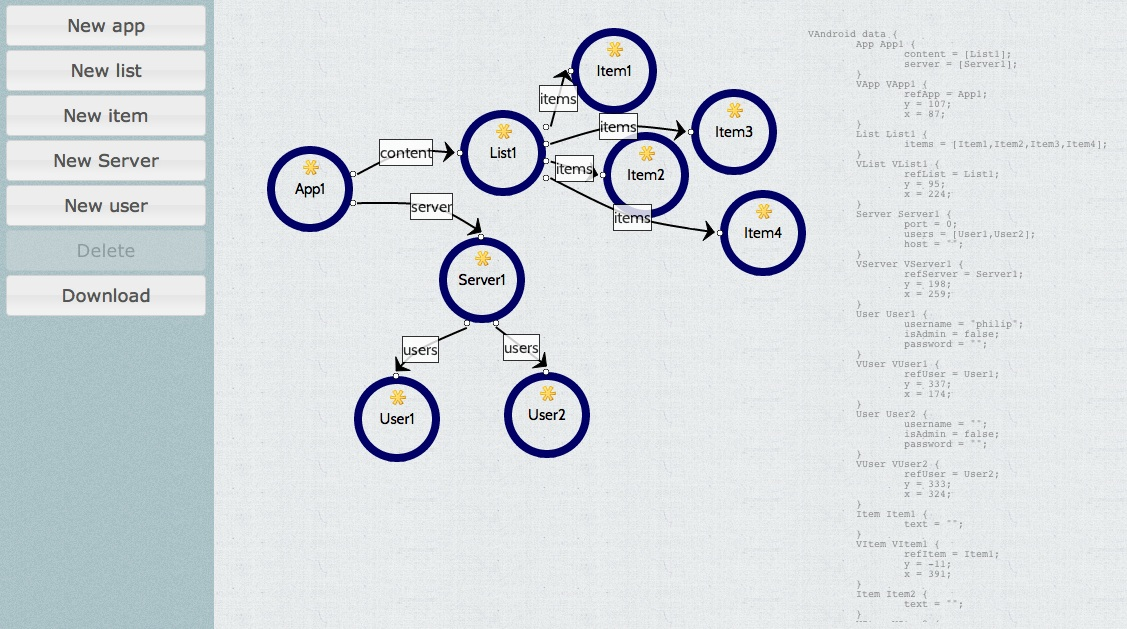
\includegraphics[width=1.0\textwidth]{images/app1_visual_environment.jpg}
\caption{Visual environment.}
\label{fig:visual_environment}
\end{figure}

\section{Creating the target model using EGL}

Now that we have created the visual editor, we can construct simple models in the domain model. After creating a model, a user can download this model, which produces a file containing Metadepth code. This Metadepth code follows the textual syntax of the domain model we created and is an instance of the \texttt{Android} model created before. The source model that contains a list component with items and a server component associated with a list of users now has to be transformed into a target model. \\ \\
One approach to transforming the source model into the target model is to use an EGL template that interweaves static code sections with dynamic code sections. The static code sections contain the \texttt{Presentation}, \texttt{Activity} and \texttt{Actions} models. The dynamic code sections are filled in with the parts found in the generated source model. For example, we use the following EGL template to construct a list component in the target model:
\begin{lstlisting}[label=target-model,caption=List component in the target model, captionpos=t]
[% for (li in app.content) { %]
	List [%= li %] {
		childActivity = "MainChildActivity";
		items = [[% for (it in li.items) { %][%= it %], [% } %]];
	}
	[% for (it in li.items) { %]
		ListItem [%= it %] {
			text = "[%= it.text %]";
			type = "MainActivity";
		}
	[% } %]
[% } %]
\end{lstlisting}
In this EGL template we iterate the \texttt{app.content} field, which is a collection of items (in the source model). These items are created on their own in a \texttt{ListItem} node, which re-uses the \texttt{text} field from the \texttt{Item} source model. Executing the complete EGL template results in a target model that is conform to the collaborative modeling framework. Using this target model, we can generate an Android binary that runs on all Android phones that have a version of 2.2 or higher.

\section{Conclusion}

Now that we have created a visual editor for the collaborative modeling framework, the barriers of entry to modeling an Android application have been lowered significantly. Although the applications that can be created using the visual environment are limited to a narrow problem domain, they allow a modeler to easily create domain specific Android applications, eliminating the need of technical knowledge.
